\chapter{Mentor Materials - Matter and Energy}

If your student has more questions about how the atomic models were developed, 
we present a brief history below. Students may also benefit from this video: 
https://youtu.be/Vf0I_2O7zUA?si=t9zbwjWoFLG8fo8o.


\subsection{Models of the Atom}
Over the history of science, there have been many ideas about the structure of
atoms. This history is a good example of how science develops: unexpected
results drive scientists to update their models, moving us closer and closer to
a true model of the atom.

During his investigations into the behavior of gases,
John Dalton (lived 1766-1844) noted that different elements combine in strict
ratios. For example, he noted that nitrogen and oxygen combine in a 1:1 and 1:2
fashion, but no ratio in between.

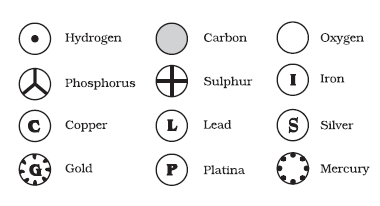
\includegraphics[width=0.75\textwidth]{daltons_model.png}

This first model of the atom is rudimentary; each element is a unique atom,
and those atoms cannot be subdivided. The atom is modeled as one large, solid, 
uniform, and neutral object. Some scientists, including the British physicist 
J.J. Thomson (1856-1940) thought that larger atoms (like lead) might be able 
to be broken down into smaller atoms (like hydrogen). Thomson had been 
experimenting with cathode-ray tubes and discovered that the these rays 
traveled much faster than thought possible for a particle the size of a 
hydrogen atom.

\includegraphics[width=1\textwidth]{cathode-ray.png}

This, combined with the observation that cathode rays could be deflected by
electrical charge, led him to postulate two things:

\begin{enumerate}
\item Atoms can be broken into parts smaller than a hydrogen atom
\item The part of atoms that composes cathode rays is negatively charged
\end{enumerate}

\begin{wrapfigure}{l}{3in}
\noindent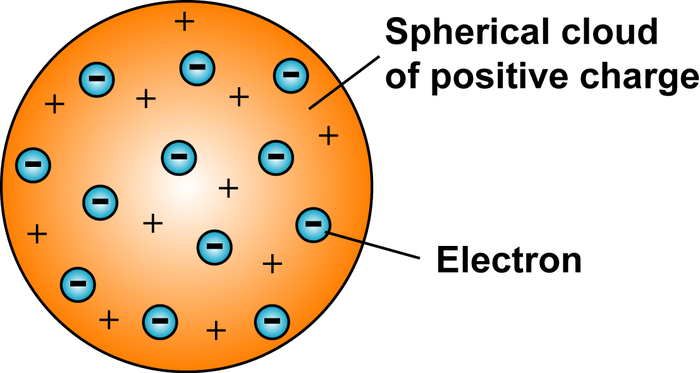
\includegraphics[width=3in]{thomson_model.png}
\end{wrapfigure}

The presence of "corpuscules" (as Thomson called them) that were negatively
charged and smaller than a hydrogen atom contradicted Dalton's theory. Thomson
updated his model of the atom, adding small, negatively charged subatomic
particles (now called electrons) that were embedded in a larger, uniform, positive
sphere. Suddenly, the atom went from neutral and indivisible to made of different
types of charged particles.

At the time, physicists were very interested in the mass-to-charge ratios of
various particles (Thomson was able to determine the mass-to-charge ratio of the
electron during his experiments), and Ernest Rutherford (1871-1937) was
investigating the mass-to-charge ratio of alpha particles. (Alpha particles, we
now know, are composed of two protons and two neutrons. They are emitted from
certain radioactive elements, including uranium.) Rutherford needed consistent
scattering of alpha particles in order to collect the data necessary to determine
the particles' mass-to-charge ratio. He achieved this by bombarding extremely
thin gold foil with alpha particles. The Thomson model of the atom would predict
that particles would be slightly deflected, as illustrated below:

\begin{center}
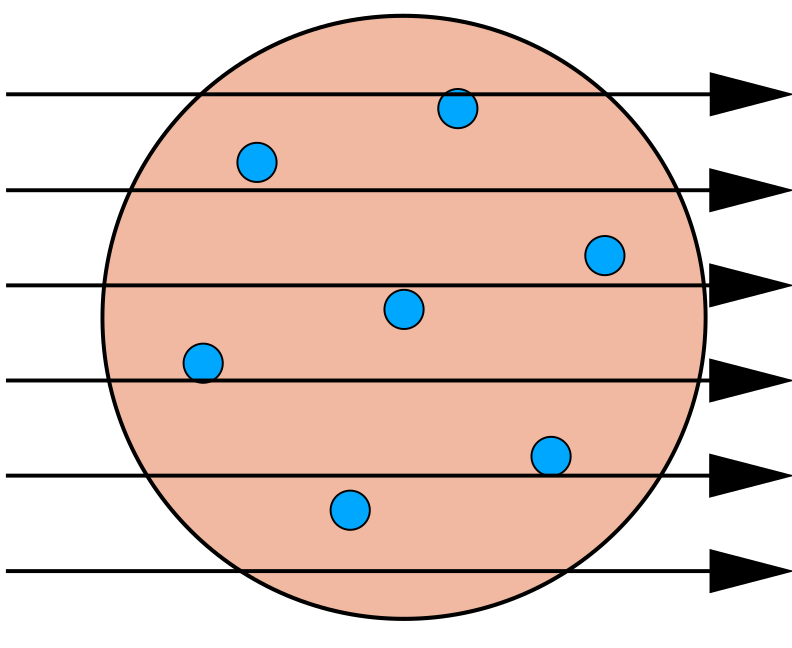
\includegraphics[width=3in]{thomson_gold.png}
\end{center}

However, a small but significant portion of the alpha particles were deflected
over $90 \deg$! To explain this, Rutherford modeled the atom as mostly empty
space with a small, dense, positive center (we now call this the nucleus).

\begin{center}
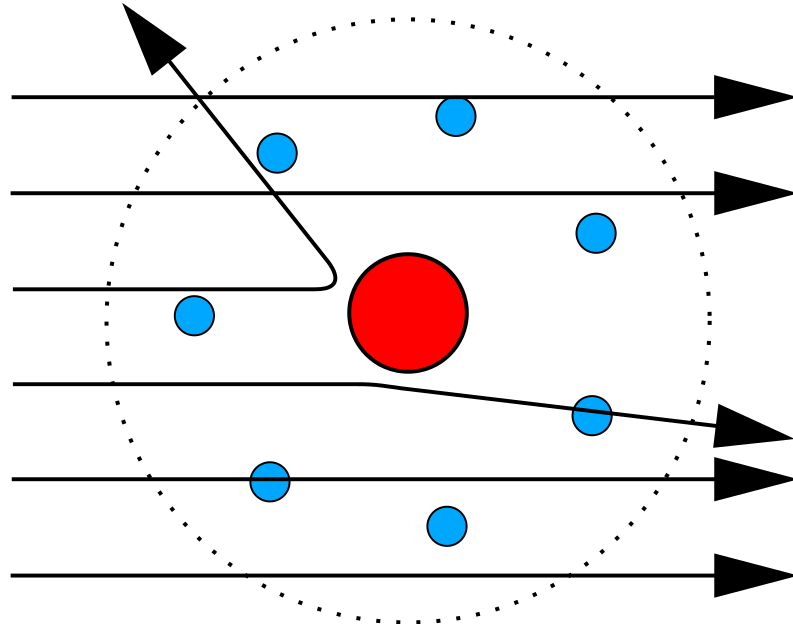
\includegraphics[width=3in]{rutherford_gold.png}
\end{center}

At the same time that Rutherford was conducting his gold foil experiments, Niels
Bohr was investigating the hydrogen line series. When hydrogen is electrically 
excited, it emits specific bands of color, not a complete spectrum. Every 
element has a unique emission spectrum. You can see the emission spectra for 
several elements below. 

\begin{center}
\noindent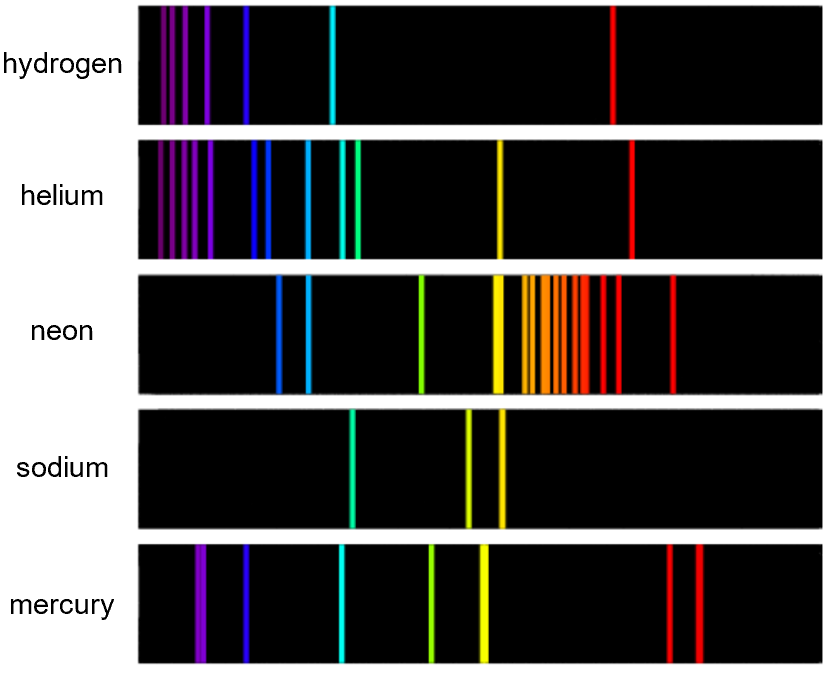
\includegraphics[width=3in]{spectral_lines.png}
\end{center}

Bohr, upon learning of Rutherford's experiments, embraced the Rutherford model 
over the Thomson model and postulated that electrons existed only at discrete 
distances from the nucleus. When electrified, a hydrogen atom's electrons 
would gain energy and "jump" up one or more levels. The electron would be 
unstable in this energized state, and eventually "fall" back to the lowest 
energy level, emitting the extra energy as light. different colors of light 
have different energies: violet being the most energetic and red being the 
least. The different levels had differing amounts of energy between them, 
resulting in only those colors corresponding to the exact energy step between 
levels being emitted. This model, called the Bohr model or the Rutherford-Bohr 
model, expands on the Rutherford model by limiting electrons to specific 
distances from the nucleus, and is often compared to a model of the solar 
system.

\begin{wrapfigure}{r}{3in}
\noindent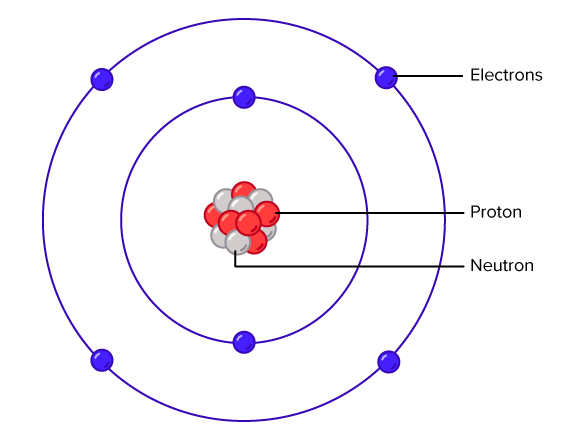
\includegraphics[width=3in]{bohr_model.png}
\end{wrapfigure}

This is likely the model you are most familiar with seeing, and it is the one we
will use most often in this text. 

However, the Bohr model is slightly inaccurate. While it is a convenient model for
thinking about atoms, in reality, electrons don't neatly orbit the nucleus.
Scientists don't know exactly where an electron will be in relation to the
nucleus, but they do know where it is most likely to be. They use a cloud that is
thicker in the center but fades out at the edges to represent an electron's
position.

\begin{wrapfigure}{l}{3in}
\noindent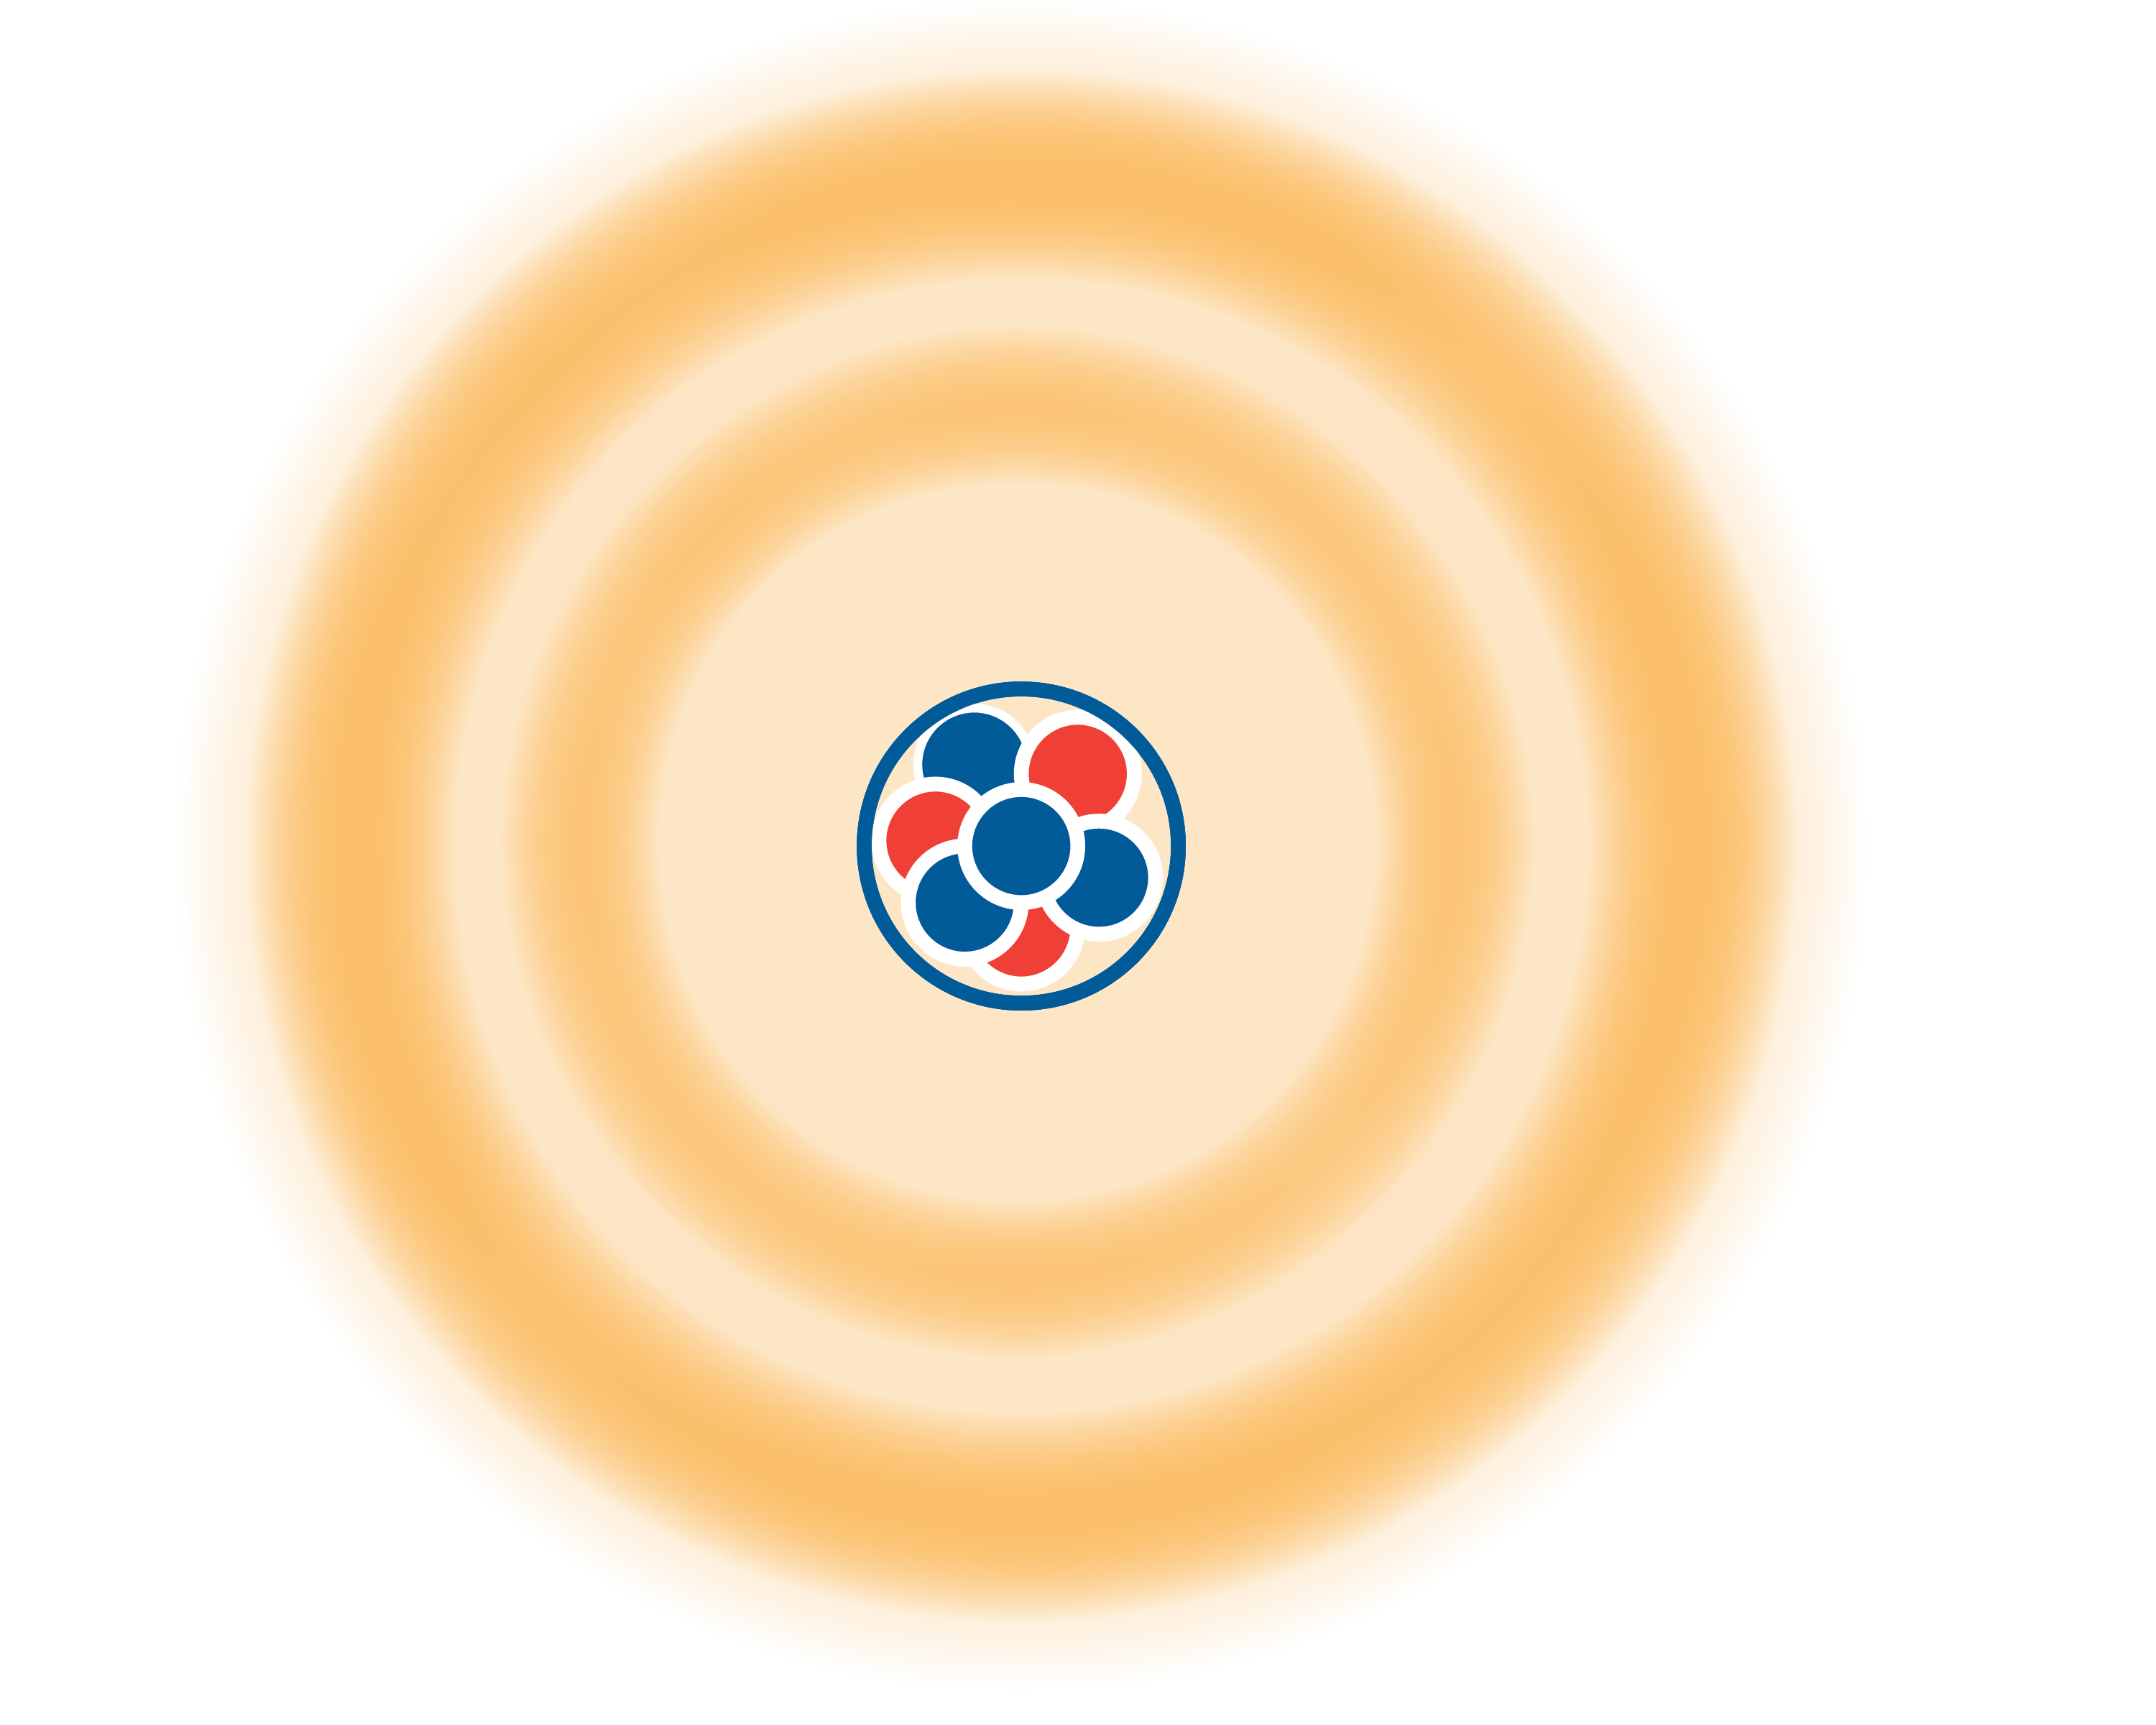
\includegraphics[trim={0 5cm 0 0}, width=3in]{atomCloud.png}
\end{wrapfigure}

\subsection{Atomic Stability}
We refer to isotopes and their stability or instability. Students can explore this concept further and create stable and unstable isotopes using the Atom Builder PhET: https://phet.colorado.edu/en/simulations/build-an-atom

\subsection{Calculating Average Atomic Mass}
If your student wants to know about more about average atomic mass before starting Sequence 2, there is a brief lesson below:

As stated above, the average atomic mass listed on the periodic table is the 
weighted average of all the isotopes of that element. Let's see how this is 
calculated for chlorine, which has 2 major isotopes: Cl-35 and Cl-37. Their 
relative abundances are shown below:

\begin{center}
\begin{tabular}{|c|c|}
\hline
Isotope & Abundance (\%)\\
\hline
Cl-35 & 75.8\%\\
\hline
Cl-37 & 24.2\%\\
\hline 
\end{tabular}
\end{center}

The relative abundance tells us what percentage of the chlorine in the universe 
is that particular isotope. For chlorine, approximately 75.8\% of all the 
chlorine in the universe is chlorine-35. Another way to think of abundances is 
this: if you had 1000 randomly-selected chlorine atoms, 758 of them would be 
Cl-35, while the remaining 242 would be Cl-37. Now for the calculation. To 
find the average atomic mass, we use the weighted average:

\begin{mdframed}[style = important, frametitle = {Calculating Average Atomic Mass}]
For an element with $n$ isotopes, each with abundance $A_i$ and mass $M_i$, the 
average atomic mass of the element is given by:

$$M_1 A_1 + M_2 A_1 + \dots +M_n A_n$$
\end{mdframed}

In the case of chlorine, there are only two isotopes:

$$35 \left(0.758\right) + 37 \left(0.242 \right) \approx 35.5$$

So the average atomic mass of chlorine is approximately 35.5 amu (atomic mass 
units). 

We can also use this equation to determine the relative abundances of elements. 
Consider boron, which has 2 stable isotopes: B-10 and B-11. According to the 
periodic table, boron's average atomic mass is 10.81. Using this information, 
we can find the relative abundances of boron-10 and boron-11. We know two 
things: the abundances of both isotopes of boron must add to 1 (or 100\%), and 
the average atomic mass. Using this, we can set up a system of equations:

$$A_{B-10} + A_{B-11} = 1$$
$$A_{B-10} \left( 10 \right) + A_{B-11} \left( 11 \right) = 10.81$$

(recall that 10 is B-10's mass and 11 is B-11's mass). We can rearrange the 
first equation to solve for $A_{B-10}$ and substitute for it in the second 
equation:

$$A_{B-10} = 1 - A_{B-11}$$
$$\left[ 1 - A_{B-11} \right] \left( 10 \right) + A_{B-11} \left( 11 \right) = 10.81$$

Now we have an equation with only $A_{B-11}$ as an unknown, and we can solve:

$$10 - 10A_{B-11} + 11A_{B-11} = 10.81$$
$$10 + A_{B-11} = 10.81$$
$$A_{B-11} = 0.81$$

Which means natural boron is approximately 81\% B-11 and 19\% B-10. 

\begin{Exercise}[title = {Finding Abundances}, label = abund]
Silicone has 3 major isotopes: Si-28, Si-29, and Si-30. If the natural 
abundance of Si-30 is 3.092\%, what are the abundances of Si-28 and Si-29? 
(Hint: use a periodic table to find the average atomic mass of silicon).
\end{Exercise}

\begin{Answer}[ref = abund]
According to the Royal Society of Chemistry, the average atomic mass of silicon 
is 28.085. [From this, we can guess that Si-28 should be the most abundant 
isotope.] We can set up a system of equations:
$$A_{Si-28} + A_{Si-29} + A_{Si-30} = 1$$
$$A_{Si-28} \left( 28 \right) + A_{Si-29} \left( 29 \right) + A_{Si-30} \left( 30 \right) = 28.085$$

We can substitute for what we already know about Si-30:
$$A_{Si-28} + A_{Si-29} = 1 - 0.03092 = 0.96908$$
$$A_{Si-28} \left( 28 \right) + A_{Si-29} \left( 29 \right) + \left( 0.03092 \right) \left(30 \right) = 28A_{Si-28} + 29A_{Si-29} + 0.9276 = 28.085$$

Now we have two equations with two unknowns:
$$A_{Si-29} = 0.96908 - A_{Si-28}$$

Substituting and solving:
$$28A_{Si-28} + 29 \left[ 0.96908 - A_{Si-28} \right] = 28.085 - 0.9276$$
$$28.10332 - A_{Si-28} = 27.1574$$
$$A_{Si-28} = 0.8758$$

So, the abundance of Si-28 is 87.58\%, and therefore the abundance of Si-29 is 
9.328\%. Notice, this answer aligns with our expectation that Si-28 is the most 
abundant isotope. 
\end{Answer}
